% P:HG1
\textbf{The alternative cover lowers complete cost.} Under common \texttt{light\_v1} measurement on the same five completed streams, G uses 12.56\% less aggregate service time than H: 18.833572 versus 21.537746 seconds over 15 pairs. G is faster in 14 pairs, and all five per-stream median ratios favor G (Figure~\ref{fig:hg_costs}). The following work analysis explains how cheaper coverage preparation offsets greater response demand.

\begin{figure}[t]
\centering
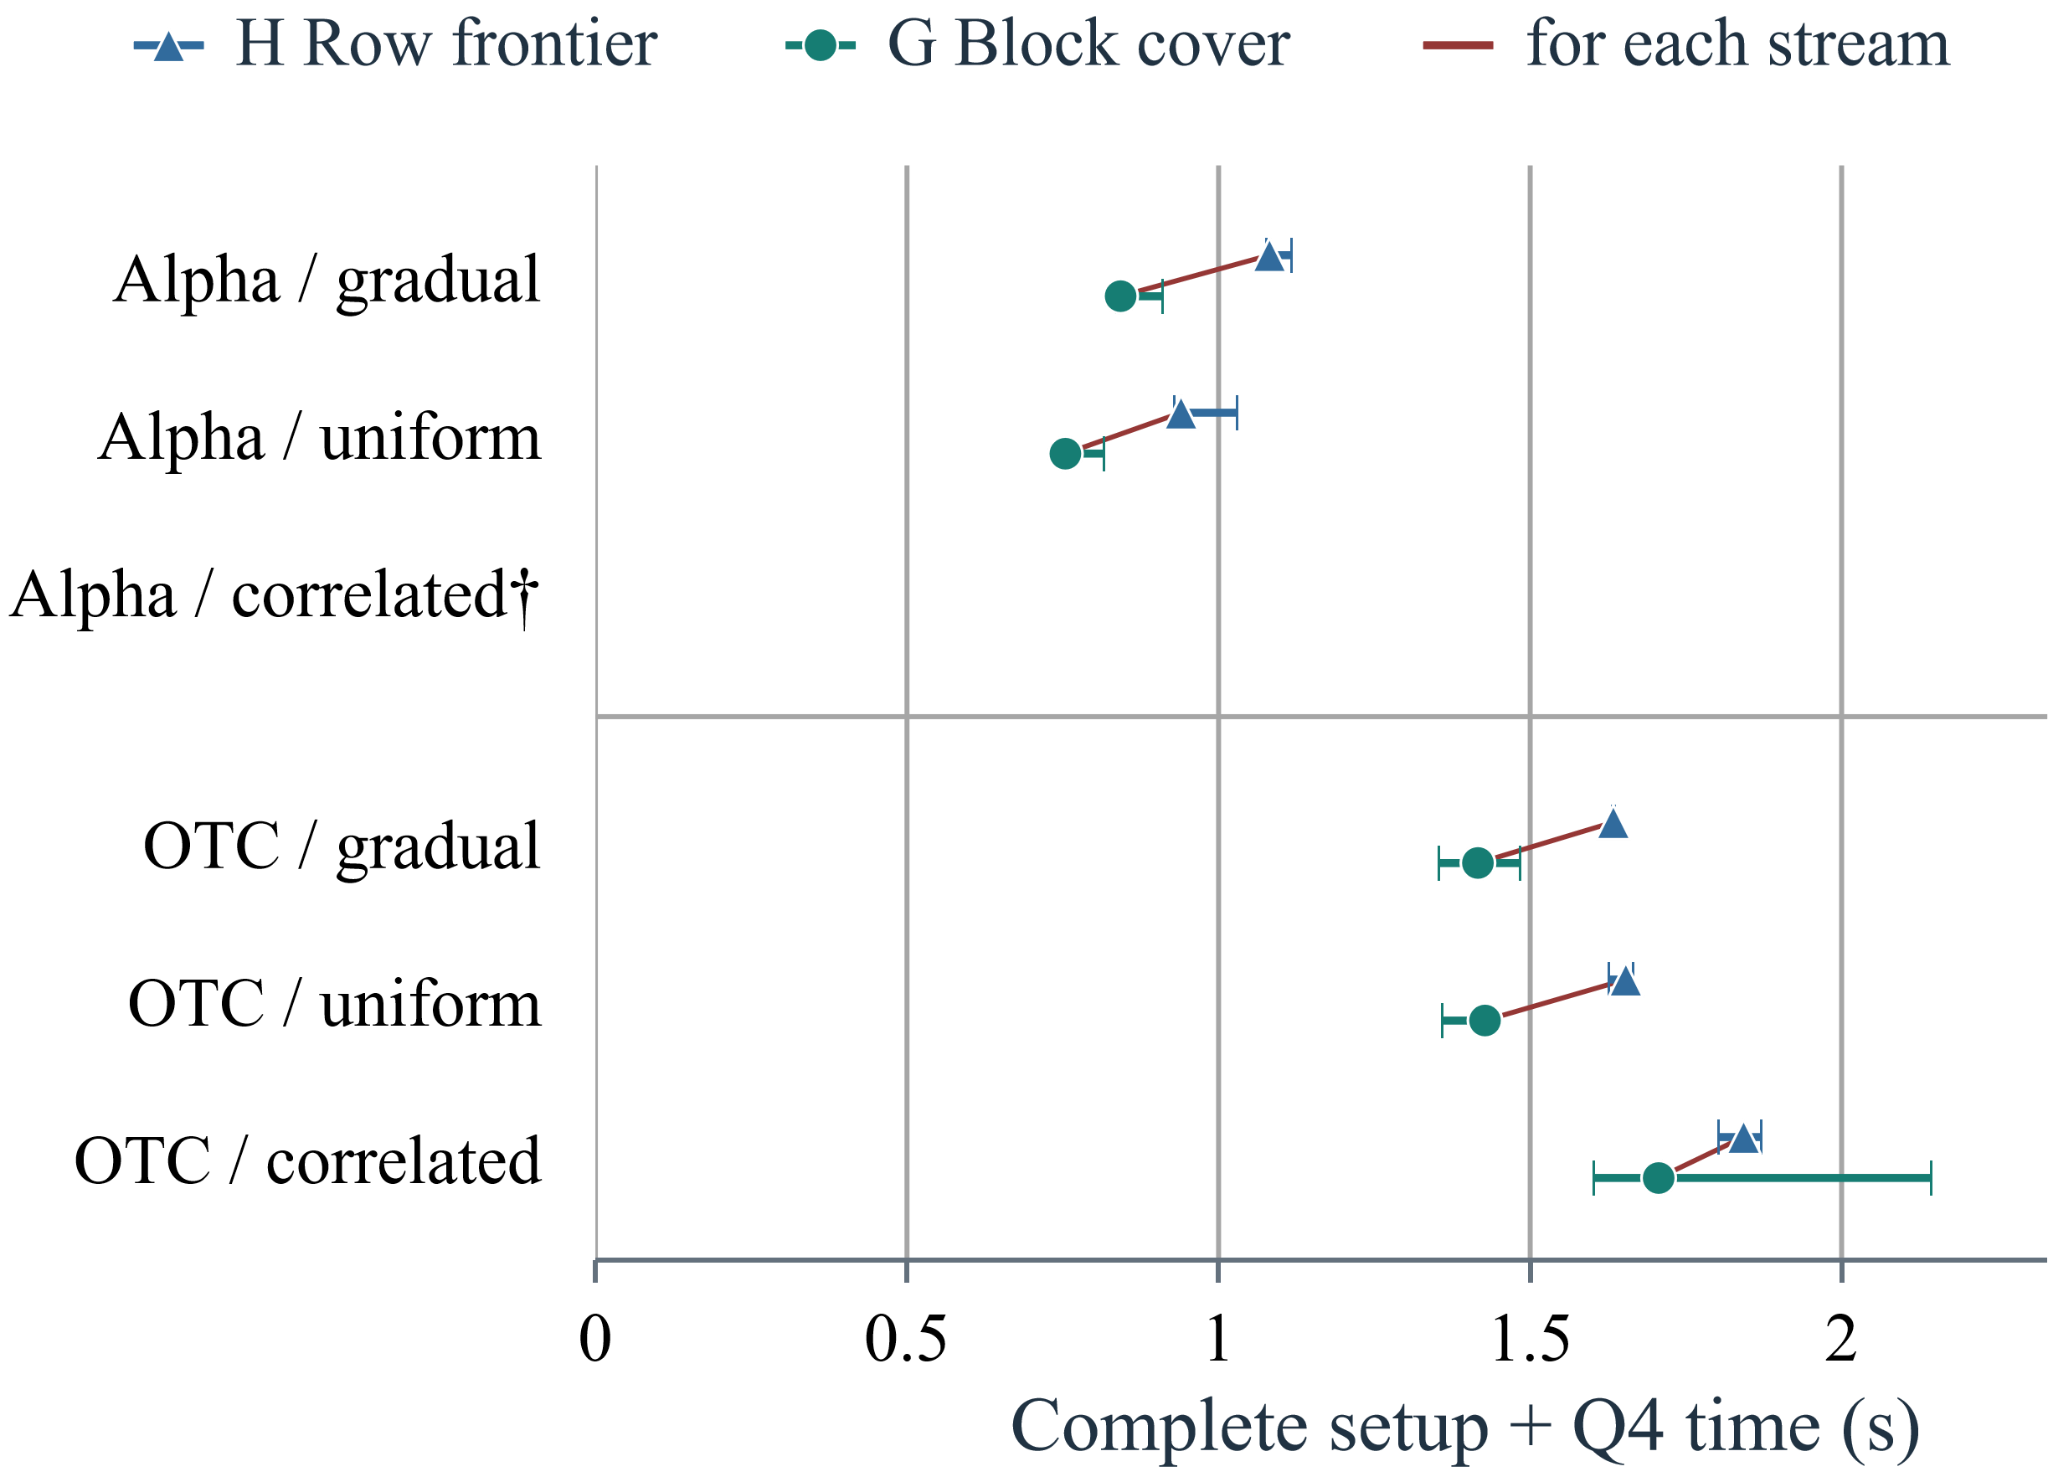
\includegraphics[width=\columnwidth]{user_originals/fig3.png}
\caption{Complete setup-plus-Q4 costs of row-frontier access (H) and block coverage (G) under common \texttt{light\_v1} measurement on the same six confirmation streams. Markers show medians; whiskers span the minimum and maximum of three timing repeats. Red segments connect H/G medians for the same stream. Opinion labels follow Figure~\ref{fig:costs}. $\dagger$ marks Alpha/correlated, for which no complete Q4 cost is available (Section~\ref{sec:completion}).}
\Description{Horizontal timing ranges compare H and G on Alpha and OTC. Blue triangles and green circles show method medians, and red segments join medians for each stream. G has a lower median in all five completed streams. The Alpha correlated stream remains as a dagger-marked row with no complete timing.}
\label{fig:hg_costs}
\end{figure}

